\chapter{Diagrama de clases}
Los diagramas de clase son una de las herramientas UML más utilizadas para el diseño de software, ya que mediante ellos se puede demostrar la manera en que interactúan las distintas clases de un programa entre sí, además de la manera de ver la manera en que interactúan con el programa.
\begin{figure}[h!]
	\centering
	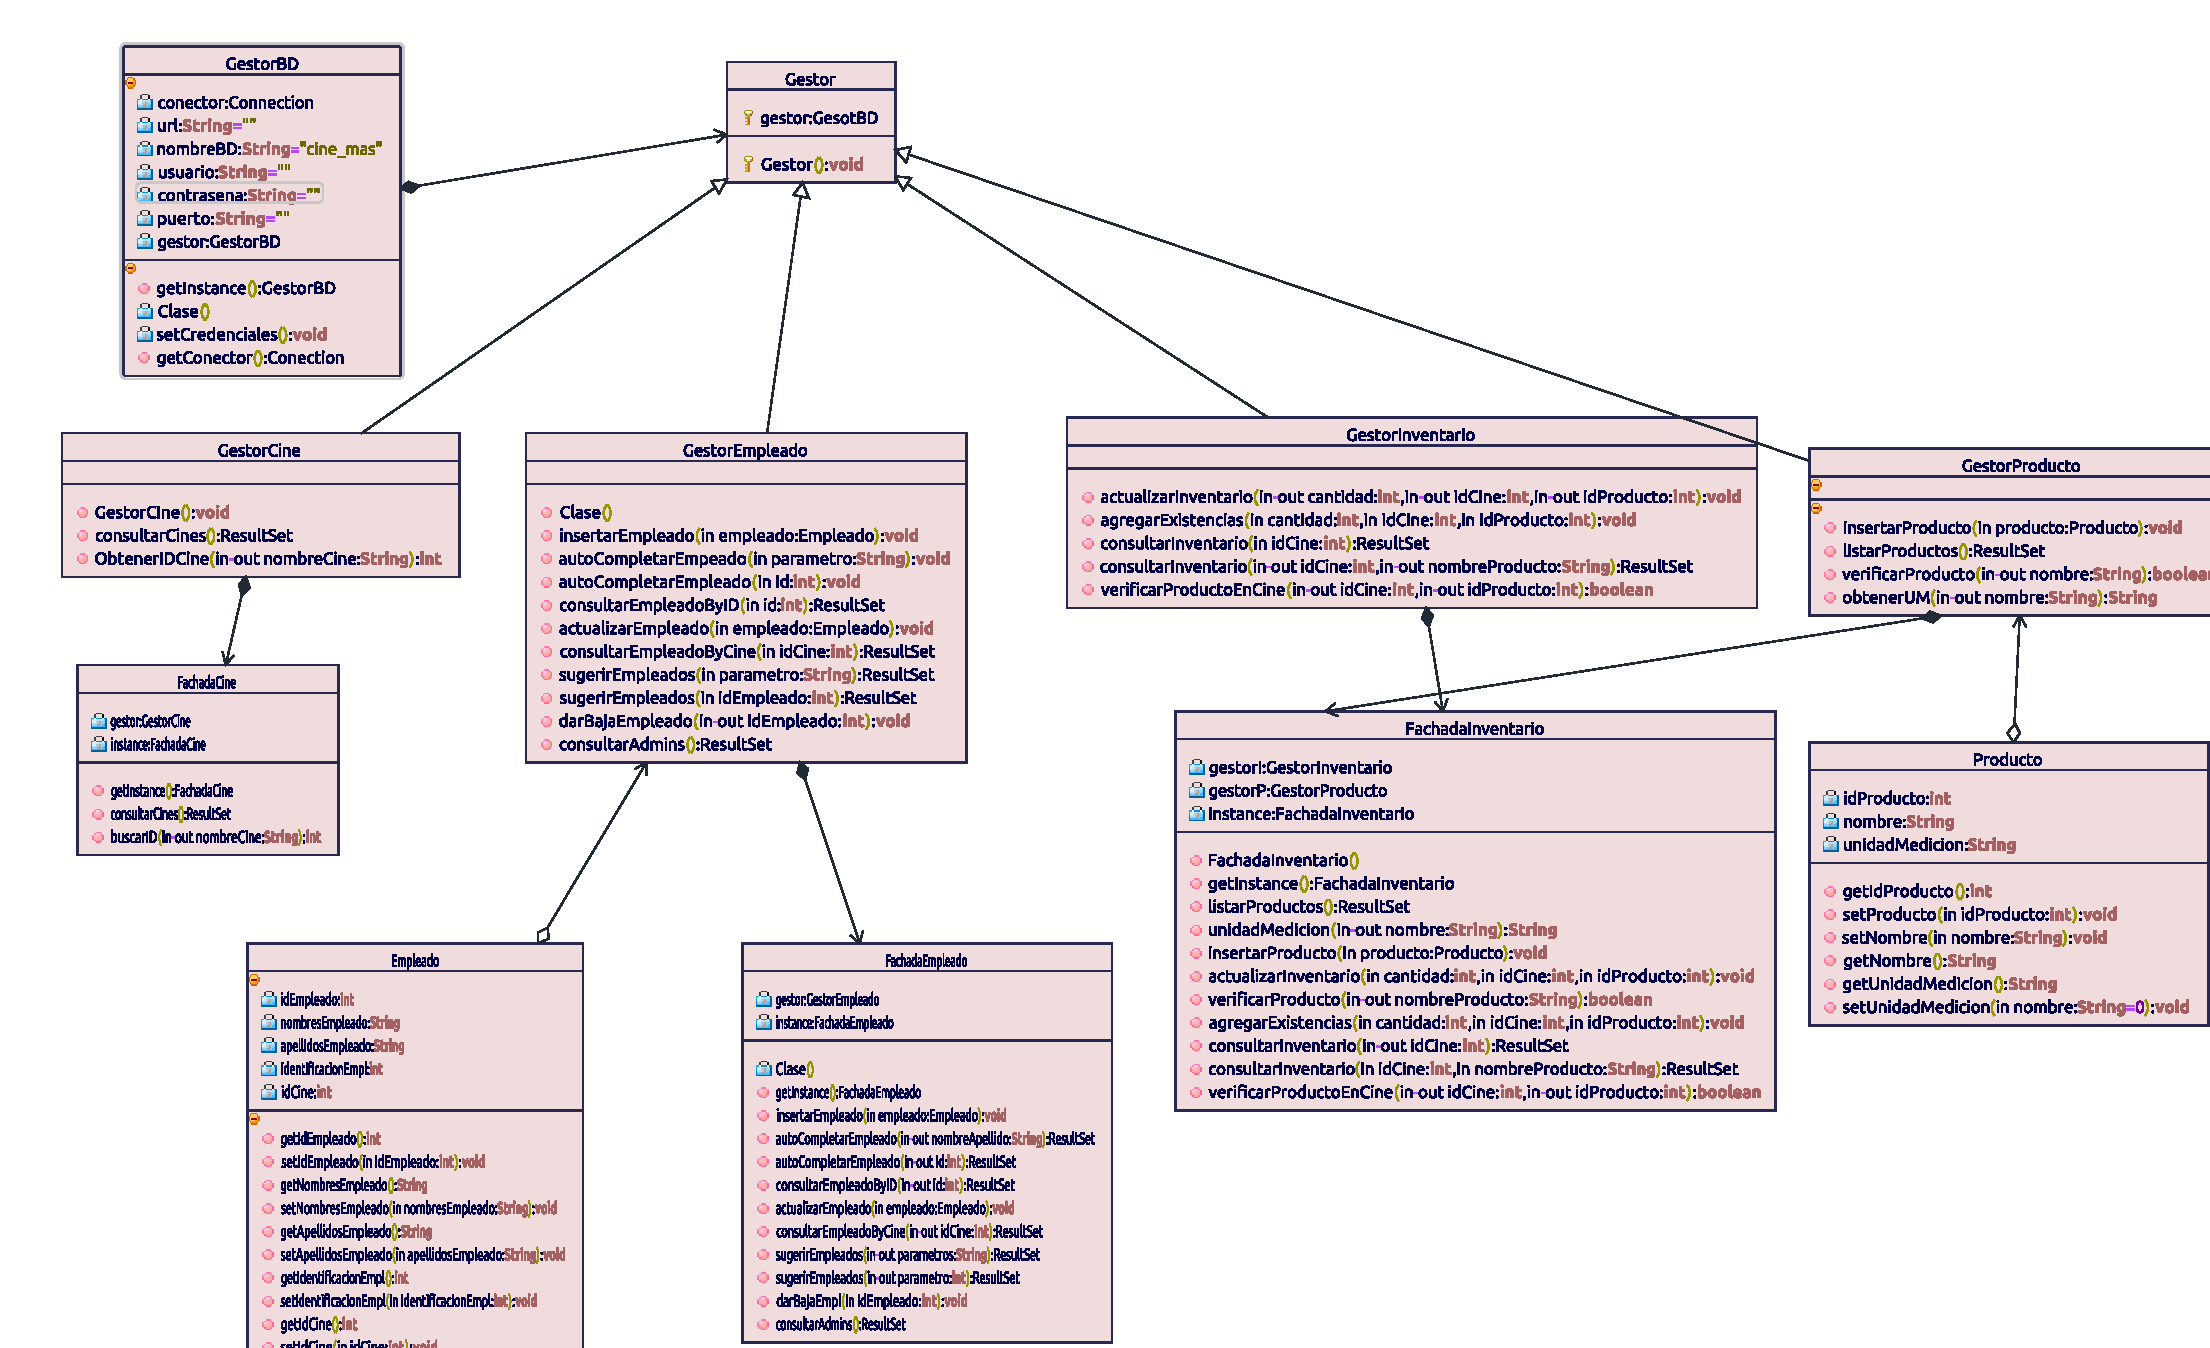
\includegraphics[scale=0.4]{diseno/clases/imgs/clases}
	\caption{Diagrama de clases}
\end{figure}
Las clases están conformadas por tres partes importantes: el nombre de clase, los atributos y las operaciones.

\subsection{NOMBRE DE CLASE:}
En esta sección es donde se define la clase, generalmente se nombran con sustantivos y se busca, mediante estos expresar de manera implícita lo que representa la clase.
  
\subsection{ATRIBUTOS}
Son las características propias de la clase, los elementos que la hacen única. Todos los atributos tienen ciertas características especiales que determinarán la manera con la que se interactúa con ellos.

\subsubsection{VISIBILIDAD}
Cuando hablamos de la visibilidad de un atributo se hace referencia a facilidad que tienen otras clases de ver los atributos de una clase en específico, existen cuatro tipos de visibilidad.

\begin{itemize}
	\item{\textbf{Privada:} este tipo hace referencia a que la única clase que tiene acceso a un atributo es la clase dueña del atributo.}
	\item{\textbf{Protegida:} este tipo está fuertemente ligado con la herencia, pues significa que los atributos son privados para todas las clases excepto aquellas que extiendan de la clase que tenga el atributo protegido.}
	\item{\textbf{Paquete:} este tipo indica que el atributo es privado para todas las clases que no pertenezcan al mismo paquete del atributo dueño del atributo. 	}
	\item{\textbf{Pública:} finalmente este tipo indica que cualquier clase existe puede ver el atributo de la clase.}
\end{itemize}

\subsubsection{ALCANCE}
Esta característica de los atributos nos indica el lugar que va a ocupar en memoria, partiendo del hecho de que en todo programa se cuenta con tres tipos de memoria: memoria estática, memoria de pila, memoria de montículo.

\begin{itemize}
	\item{\textbf{Memoria estática:} Esto nos indica que un atributo no puede cambiar en tiempo de ejecución, es decir, siempre tendrá el mismo valor.}
	\item{\textbf{Memoria de pila:} la mayoría de los atributos se encuentra en esta memoria, son datos que cambian constantemente.}
	\item{\textbf{Memoria de montículo} En esta memoria se encuentran todos los atributos que necesitan ser instanciados, generalmente con la palabra reservada \textbf{new}}
	
\end{itemize}

\subsubsection{PROPIEDADES}
Esta característica de los atributos es lo que nos indica la posibilidad que se tiene de ser modificados en tiempo de ejecución, se tienen de do tipos: Final y volátil.

\begin{itemize}
	\item{\textbf{Final o Constante:} ste tipo de atributo es un atributo que una vez definido no puede ser modificado en tiempo de ejecución.}
	\item{\textbf{Volátil:} Por otro lado esta propiedad indica que el atributo puede ser optimizado en tiempo de ejecución.}
\end{itemize}

La definición de un atributo dentro de una clase se realiza de la siguiente manera:

\centerline{\textbf{\underline{Visibilidad nombre [ ]: tipo = valor {propiedad}}}}
Donde los “[ ]” hacen referencia a la cantidad de elementos que se tienen y el subrayado al alcance que tienen dichos atributos.



\subsection{OPERACIONES}
Cuando se habla de las operaciones de una clase se hace referencia a las “habilidades” que esta tiene para poder interactuar con el programa, al igual que los atributos tiene ciertas características que las diferencian las unas de las otras.


\subsubsection{VISIBILIDAD}
La visibilidad de una operación es muy parecida con la visibilidad de los atributos, con la diferenciación de que en general solo cuenta con visibilidad pública y privada. 

Para saber si una operación es pública o privada hay que tener un término que se llama cohesión secuencial, es decir, si la operación necesita de otras operaciones para funcionar correctamente.

Una operación es privada si dicha operación  realiza una actividad que solamente tiene sentido dentro de la clase.

una operación es pública si la operación permite la interacción con otras clases. Generalmente dentro de ella aparece la cohesión secuencial, es decir, ella llama a las operaciones privadas de la clase. Se denomina interfaz, pues es un mediador con otras clases.


\subsubsection{PROPIEDADES}
En el caso de las operaciones las propiedades indican el tipo de acción que permite realizar.

\begin{itemize}
	\item{\textbf{Final: }La operación no permite sobrecarga, es decir, las clases hijas no podrán utilizarla.}
	\item{\textbf{Query: }Es una operación que no permite modificaciones, los atributos de la clase no son modificables.}
	\item{\textbf{Modify: }indica que la operación tiene la habilidad de modificar de manera permanente los atributos de la clase.}
	\item{\textbf{Synchronized: }Esta propiedad tiene sentido cuando se habla de hilos, pues determina que un hilo no pasará la responsabilidad hasta no haber terminado el proceso.}
\end{itemize}


\subsubsection{PARÁMETROS}
Los parámetro son la información que recibe la operación para poder realizar el proceso asignado, tienen una dirección que indica la característica del atributo:

\begin{itemize}
	\item{\textbf{in:} El atributo se pasa por valor.}
	\item{\textbf{out:} el parámetro será retornado.}
	\item{\textbf{in-out:} el parámetro se pasa por referencia. }
\end{itemize}

La manera en que se escriben las operaciones dentro de una clase es la siguiente:

\centerline{\textbf{\underline{Visibilidad nombre (parámetros): retorno {propiedad}}}}


\subsection{RELACIONES}
Estas relaciones tienen la característica de tener reuso de caja negra, es decir que las clases que se relacionan mediante ellas no tienen conocimiento de cómo se lleva a cabo una operación, pero aún así pueden hacer uso de ellas. Por otro lado, tienen el problema de que tienen un acoplamiento muy alto, lo que significa que la necesidad entre las clases es algo muy elevado.

\subsubsection{Cliente/proveedor}
Estas relaciones se dividen en dos grandes subramas: Dependencias y Asociaciones.

\textbf{Dependencia:}
Estos casos se dan cuando una clase utiliza otra clase para poder llevar a cabo una función (include, call, instance of, etc).

\textbf{Asociación:}
Esta tiene de dos tipos, el primero, la agregación, indica que la relación entre ellos no es vital, es decir, el cliente puede vivir sin el proveedor. Por otro lado la composición indica una relación vital, es decir, el cliente no puede vivir, ni tener sentido a no ser que tenga al proveedor.


\subsubsection{Generalización/Implementación}
Estas relaciones tienen la característica de tener reuso de caja blanca, es decir que las clases que se relacionan mediante ellas  tienen conocimiento de cómo se lleva a cabo una operación, e incluso pueden llegar a modificarlo. Por otro lado, tienen la ventaja de que tienen un acoplamiento muy bajo, lo que significa que la necesidad entre las clases es algo que puede pasar a segundo plano.

Por un lado las generalizaciones permiten crear una clase a partir de otra, con las mismas características, pero con la idea de que tenga un rol diferente. Por otro lado las implementaciones indican el uso de algunas operaciones de una interfaz en una clase determinada.

\begin{figure}[h!]
	\centering
	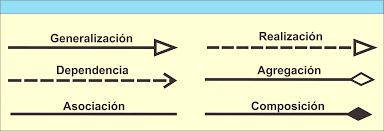
\includegraphics[scale=0.4]{diseno/clases/imgs/relaciones}
	\caption{Relaciones entre clases}
\end{figure}
